%%%%%%%%%%%%%%%%%%%%%%%%%%%%%%%%%%%%%%%%%%%%%%%%%%%%%%%%%%%%%%%%%%%%%%
%%                     Inhibition
%%%%%%%%%%%%%%%%%%%%%%%%%%%%%%%%%%%%%%%%%%%%%%%%%%%%%%%%%%%%%%%%%%%%%%

\subsection{Glyph: \glyph{Inhibition}}\label{sec:inhibition}
%\color{blue}

An inhibition \textbf{negatively} affects the flux of a process represented by the target transition. This inhibition can be for instance a competitive inhibition or an allosteric inhibition. 

\begin{glyphDescription}
 \glyphSboTerm SBO:0000169 ! inhibition.
 \glyphOrigin Any \glyph{EPN} (\sect{EPNs}) or any \glyph{logical operator} (\sect{logic}).
 \glyphTarget Any \glyph{process node} (\sect{PNs}).
 \glyphNode The target extremity of an \glyph{inhibition} carries a bar perpendicular to the arc.
 \end{glyphDescription}

\begin{figure}[H]
  \centering
  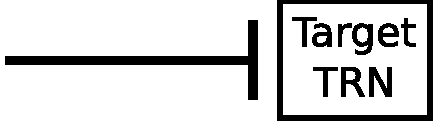
\includegraphics[scale = 0.5]{images/inhibition}
  \caption{The \PD glyph for \glyph{inhibition}.}
  \label{fig:inhibition}
\end{figure}

